% -*- latex -*-
%%%%%%%%%%%%%%%%%%%%%%%%%%%%%%%%%%%%%%%%%%%%%%%%%%%%%%%%%%%%%%%%
%%%%
%%%% This TeX file is part of the tutorial
%%%% `Introduction to the PETSc library'
%%%% by Victor Eijkhout, eijkhout@tacc.utexas.edu
%%%%
%%%% copyright Victor Eijkhout 2012-2020
%%%%
%%%%%%%%%%%%%%%%%%%%%%%%%%%%%%%%%%%%%%%%%%%%%%%%%%%%%%%%%%%%%%%%

\sectionframe{A word about SPMD parallelism}

\frame{\frametitle{Computers when MPI was designed}
  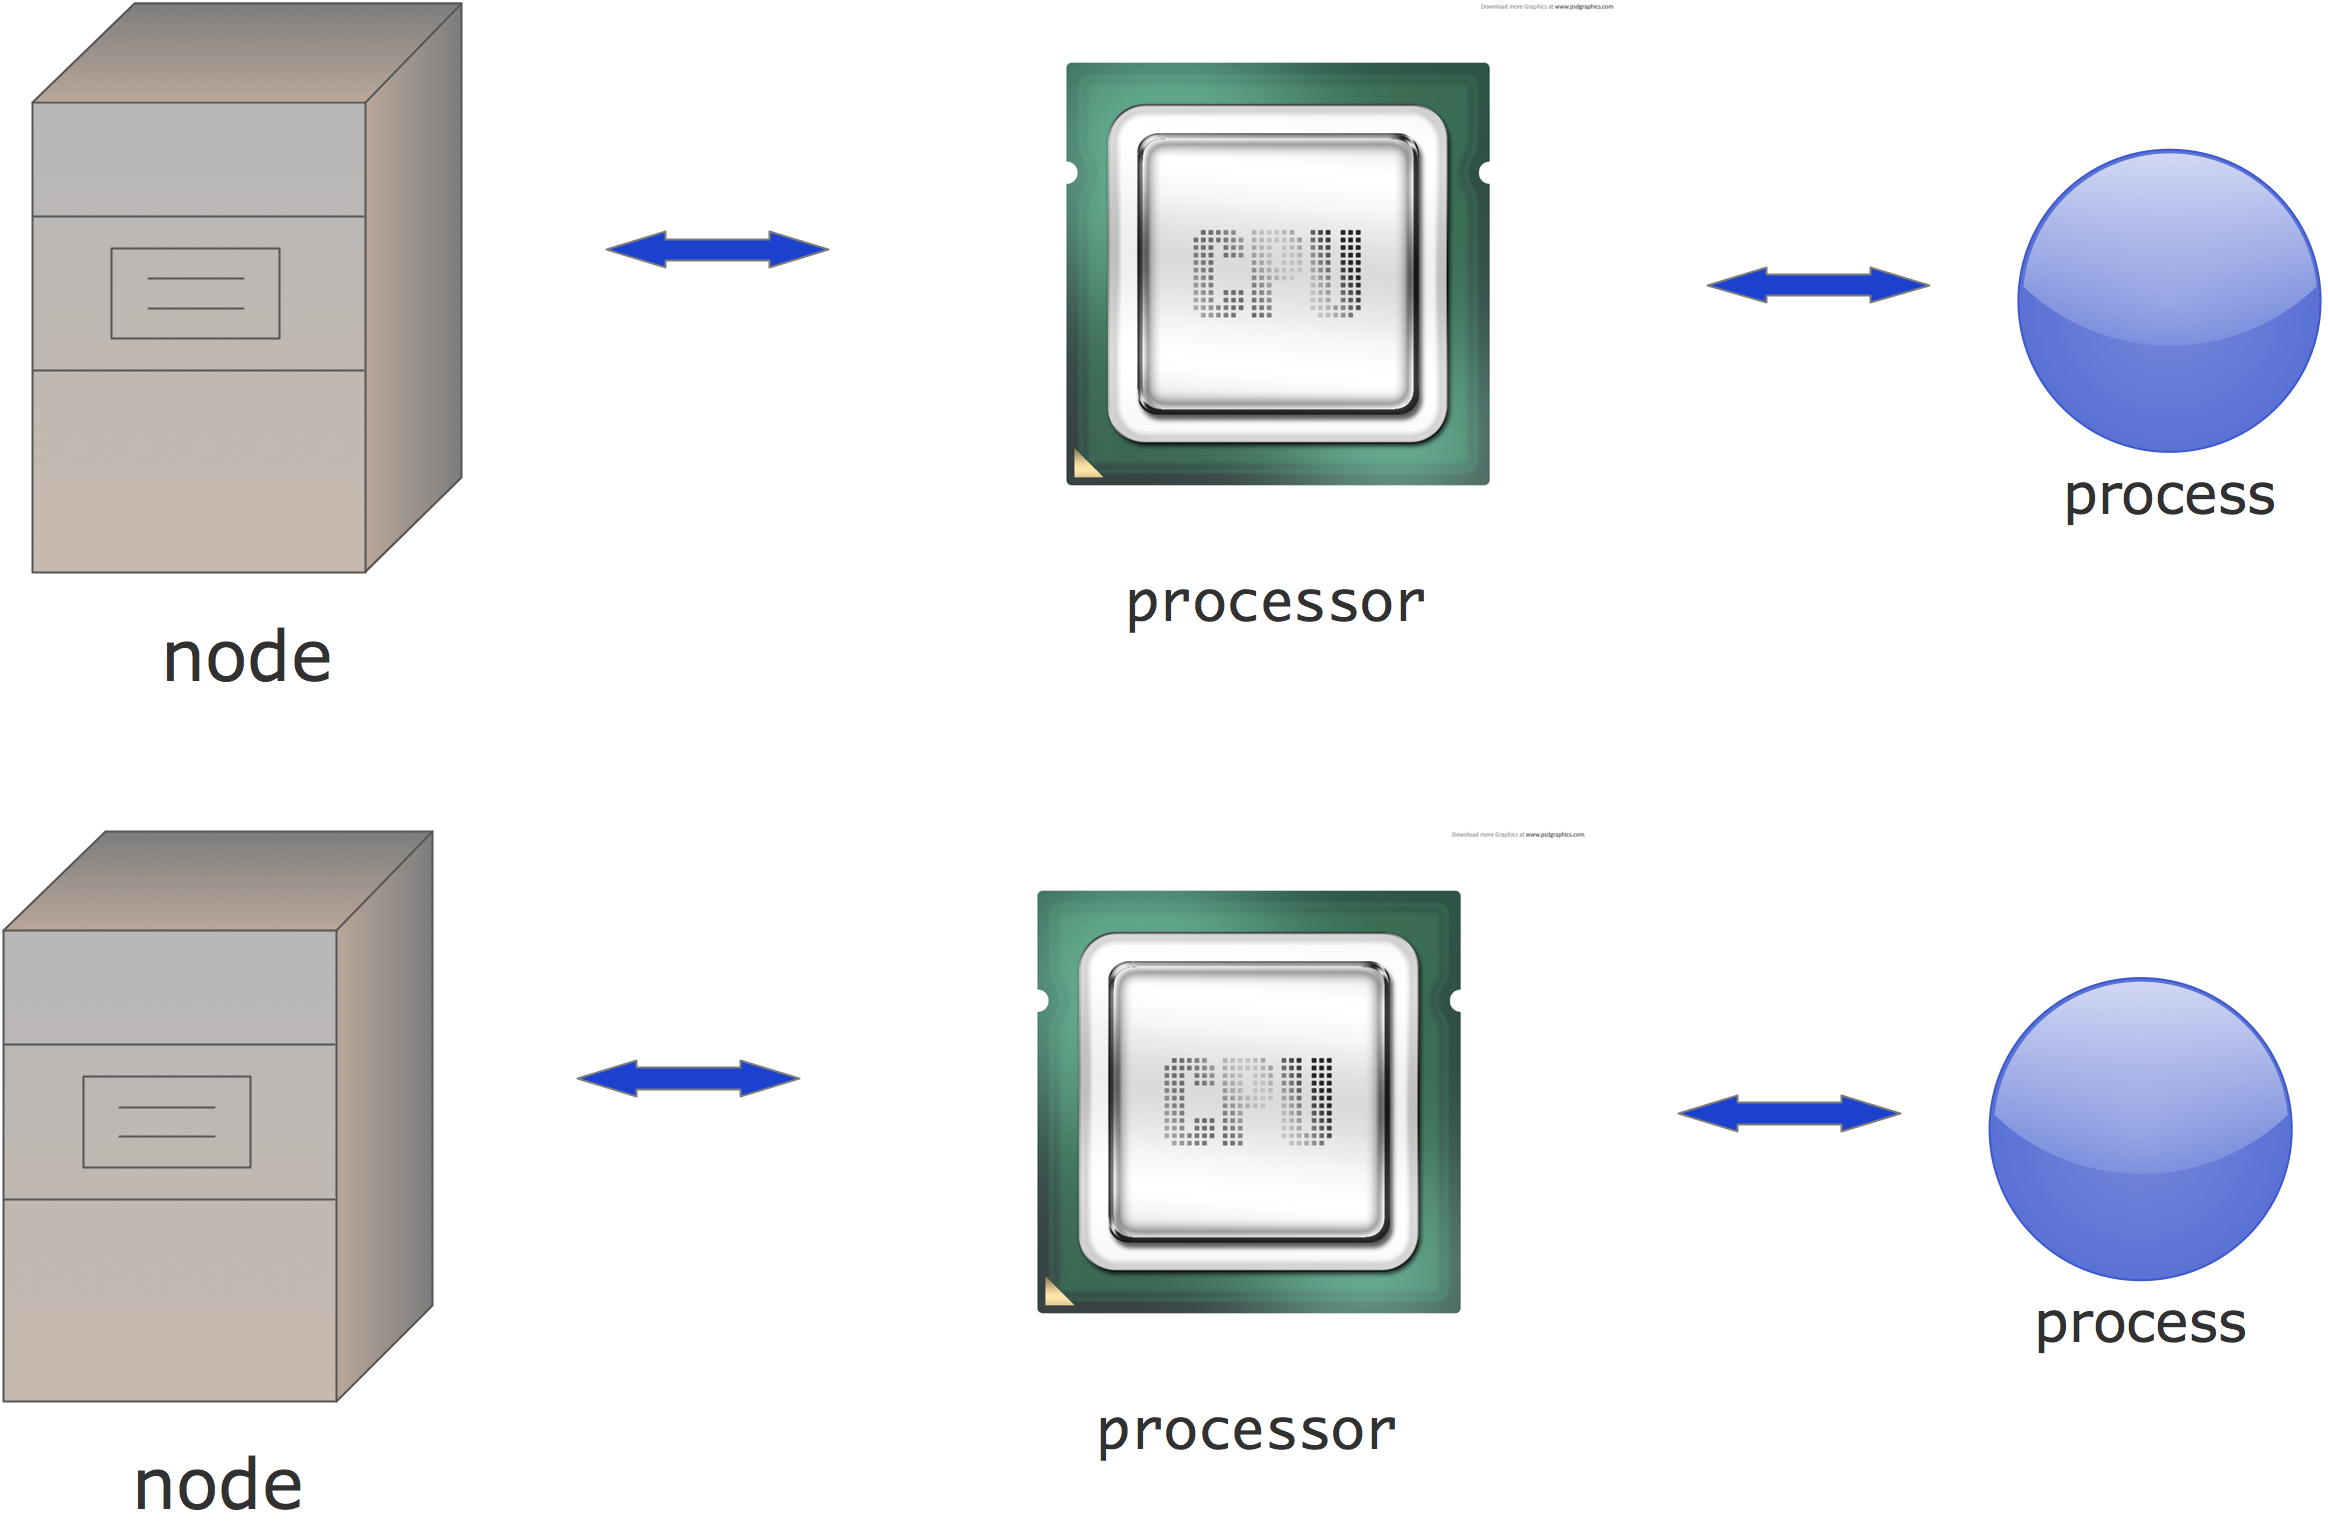
\includegraphics[scale=.1]{mpi-node1}

  One processor and one  process per node;\\
  all communication goes through the network.
}

\frame{\frametitle{Pure MPI}
  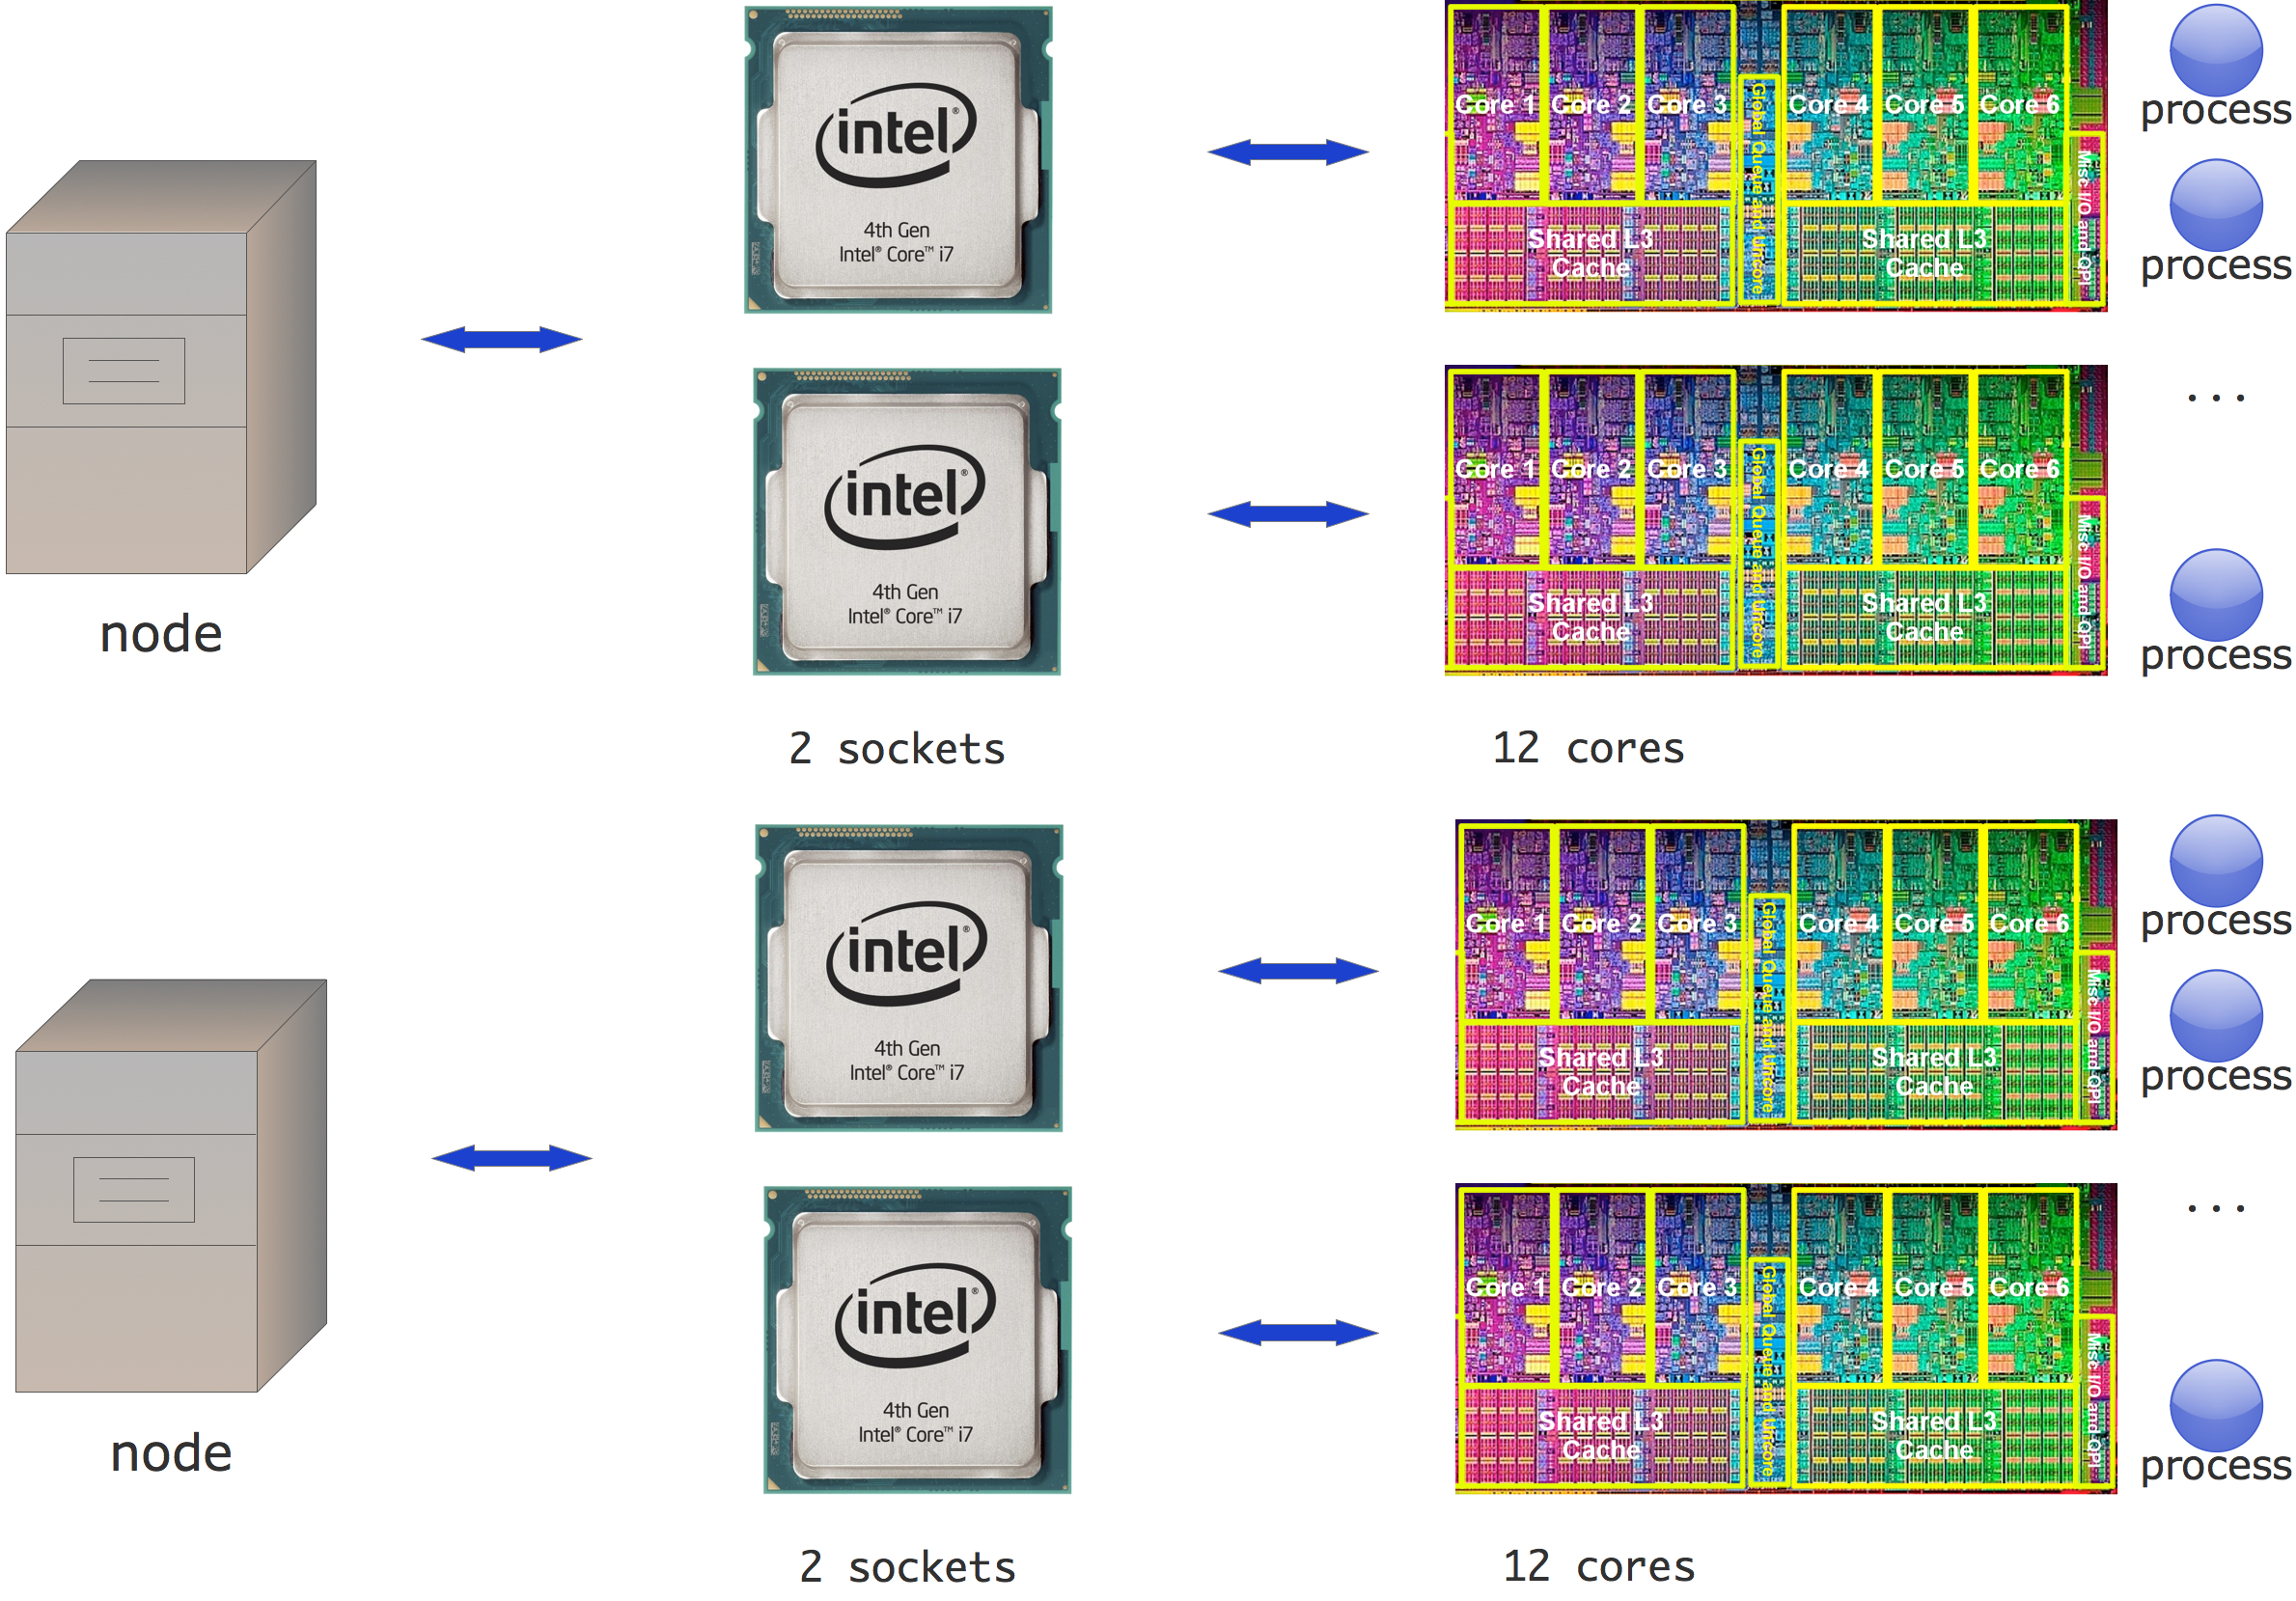
\includegraphics[scale=.06]{mpi-node2}

  A node has multiple sockets, each with multiple cores.\\
  Pure MPI puts a process on each core: pretend shared memory doesn't exist.
}

\frame{\frametitle{Hybrid programming}
  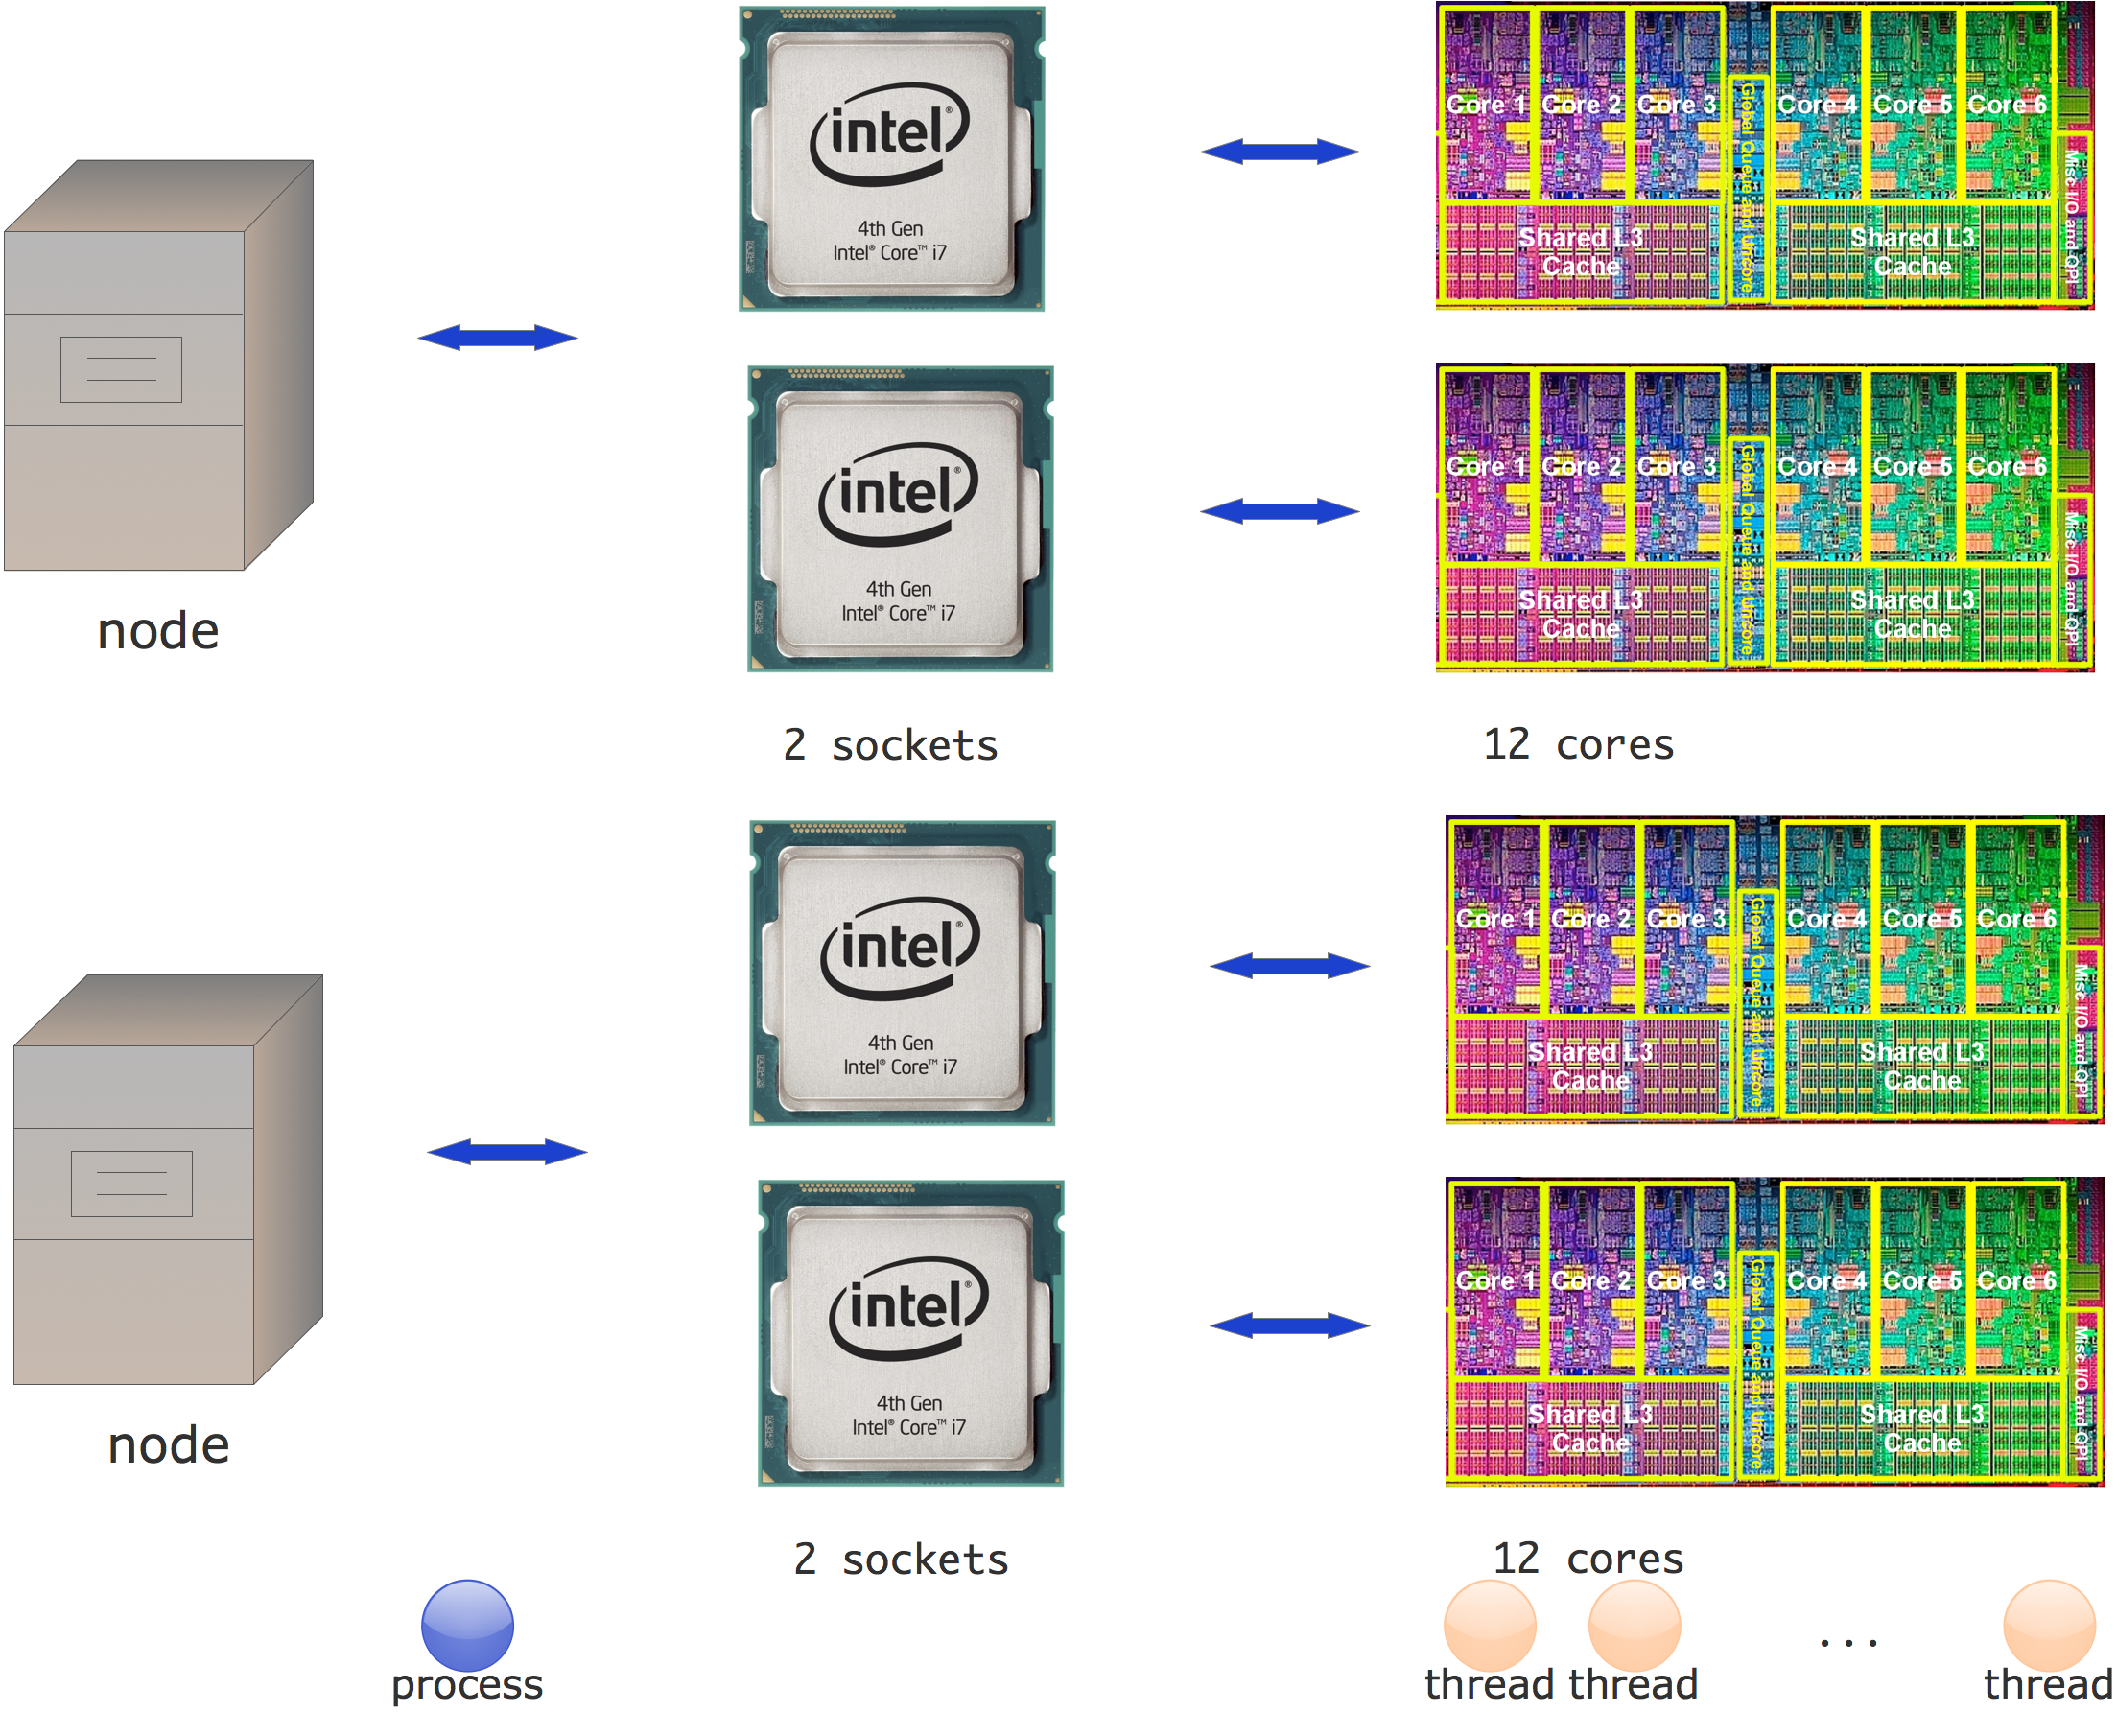
\includegraphics[scale=.06]{mpi-node3}

  Hybrid programming puts a process per node or per socket;\\
  further parallelism comes from threading.\\
  No use of threading in PETSc
}

\begin{frame}{Multi-mode programming in PETSc}
  PETSc is largely aimed at MPI programming; however
  \begin{itemize}
  \item You can of course use OpenMP in between PETSc calls;
  \item there is suppose for GPUs
\begin{taccnote}
At the moment only on frontera: \n{module load petsc/3.12-rtx}.
\end{taccnote}
  \item OpenMP can be used in external packages.
  \end{itemize}
\end{frame}

\begin{frame}{Terminology}
  `Processor' is ambiguous: is that a chip or one independent
  instruction processing unit?
  \begin{itemize}
  \item Socket: the processor chip
  \item Processor: we don't use that word
  \item Core: one instruction-stream processing unit
  \item Process: preferred terminology in talking about MPI.
  \end{itemize}  
\end{frame}

\frame{\frametitle{SPMD}
  The basic model of MPI is\\
  `Single Program Multiple Data':\\
  each process is an instance of the same program.

  Symmetry: There is no `master process', all processes are equal,
  start and end
  at the same time.

  Communication calls do not see the cluster structure:\\
  data sending/receiving is the same for all neighbours.
}

\begin{frame}[containsverbatim]{Compiling and running}
  MPI compilers are usually called \texttt{mpicc},
  \texttt{mpif90}, \texttt{mpicxx}.

  These are not separate compilers,
  but scripts around the regular C/Fortran compiler. You can use all
  the usual flags.

  At TACC:\\
  \verb+ibrun yourprog+\\
  the number of processes is determined by SLURM.
\end{frame}

\begin{frame}[containsverbatim]{Do I need a supercomputer?}
  \begin{itemize}
  \item With \n{mpiexec} and such, you start a bunch of processes that
    execute your PETSc program.
  \item Does that mean that you need a cluster or a big multicore?
  \item No! You can start a large number of processes, even on
    your laptop. The OS will use `time slicing'.
  \item Of course it will not be very efficient\ldots
  \end{itemize}
\end{frame}

\begin{frame}{Cluster setup}
  \small
  Typical cluster:
  \begin{itemize}
  \item Login nodes, where you ssh into; usually shared with 100 (or
    so) other people. You don't run your parallel program there!
  \item Compute nodes: where your job is run. They are often exclusive
    to you: no other users getting in the way of your program.
  \end{itemize}
  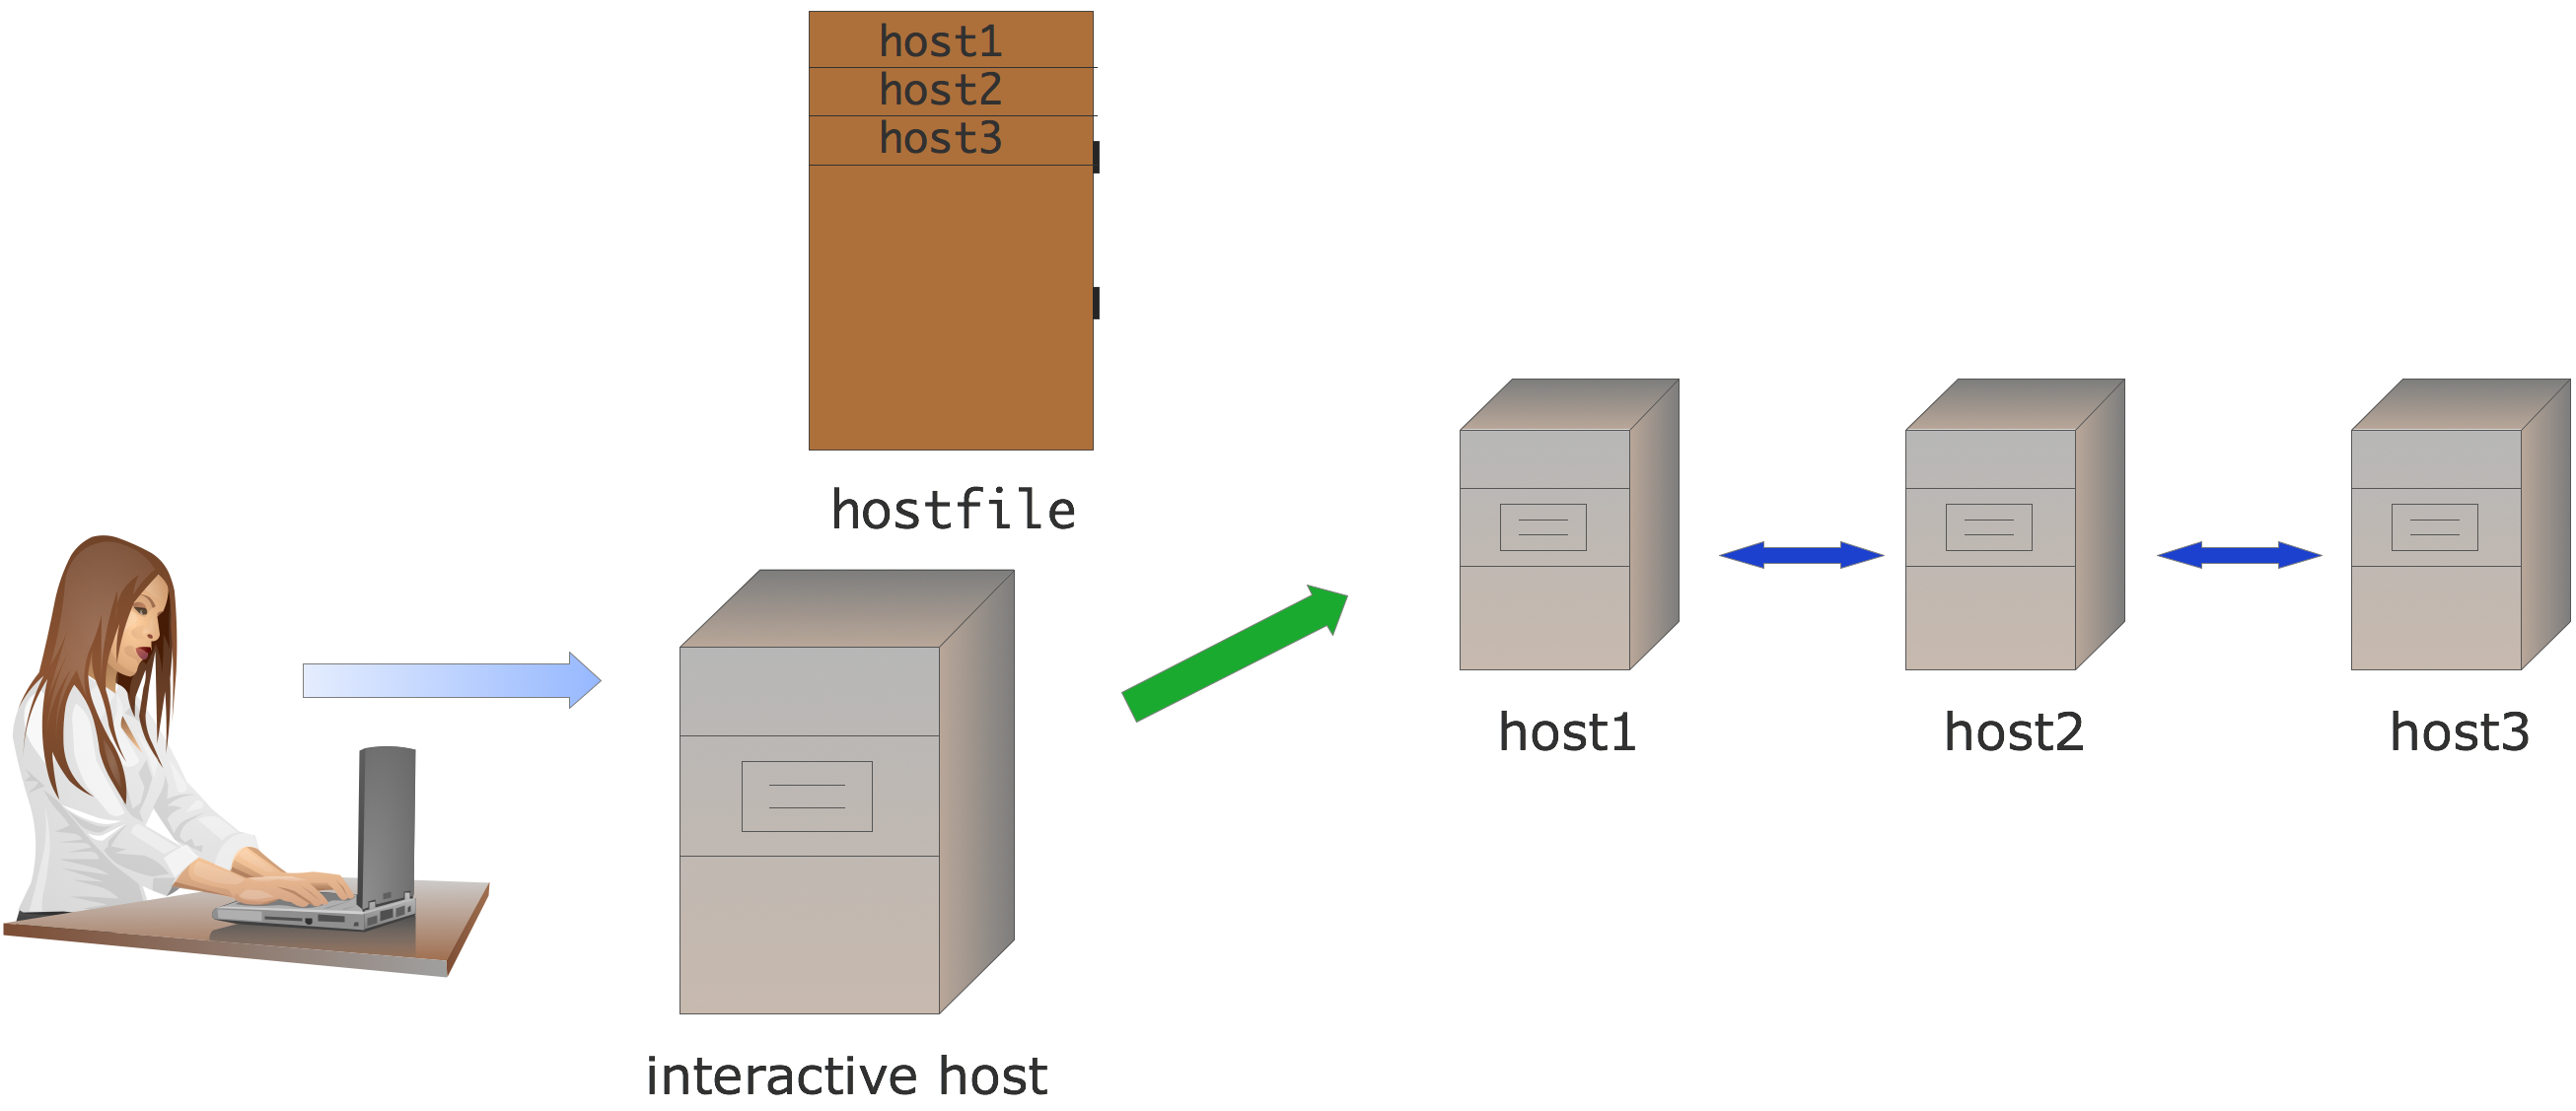
\includegraphics[scale=.08]{mpi-interactive}

  Hostfile: the description of where your job runs. Usually generated
  by a job scheduler.
\end{frame}

\begin{frame}{In a picture}
  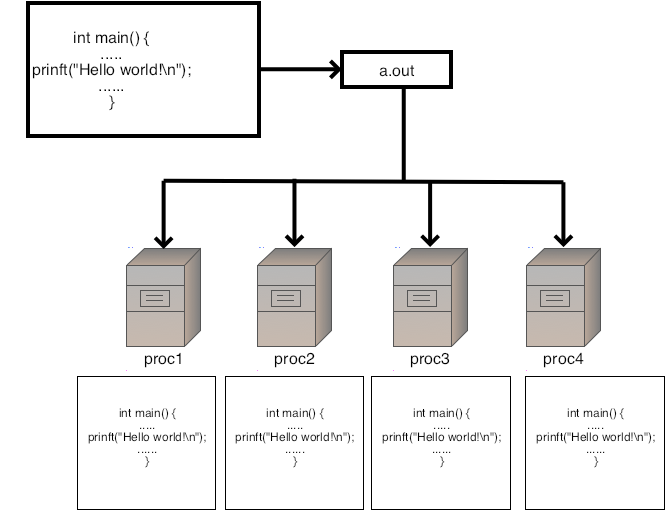
\includegraphics[scale=.3]{hello-parallel}
\end{frame}

\begin{frame}[containsverbatim]\frametitle{Process identification}
  \label{sl:ranksize}
  Every process has a number (with respect to a communicator)
\begin{verbatim}
int MPI_Comm_rank( MPI_Comm comm, int *procno )
int MPI_Comm_size( MPI_Comm comm, int *nprocs )
\end{verbatim}
For now, the communicator will be \n{MPI_COMM_WORLD}.

Note: mapping of ranks to actual processes and cores is not predictable!
\end{frame}

